\documentclass{exam}
\usepackage{graphicx} 


%Format Header and footer
\pagestyle{headandfoot}
\header{\footnotesize Klass:\\Namn:}{\Large\textbf{DNA och RNA: roll och funktion}}{\footnotesize 2025\\Viktor Arohlén}
\headrule
\footrule
\setlength{\columnsep}{0.25cm}
%\setlength{\columnseprule}{1pt}
\footer{}{Sida \thepage}{}
%\extrafootheight{-2cm}

\begin{document}
\section*{Instruktioner}
Provet består av två delar \\
    - Kryssfrågor, endast ett alternativ är rätt om inget annat anges (\textit{15 poäng})\\
    - Fördjupande frågor, svara mer omfattande (\textit{12 poäng})

\subsection*{Poäng}
Antalet poäng är markerat för varje fråga. Totalt \textbf{19 frågor} och \textbf{27 poäng}.\\ \textit{För godkänt resultat krävs 11 poäng.}

\vspace{5mm} %5mm vertical space
\begin{center}
\fbox{\fbox{\parbox{6in}{\centering
\textbf{15 kryssfrågor}: markera endast ett alternativ, om inget annat anges. (\textbf{15 poäng})
}}}
\end{center}
\vspace{5mm} %5mm vertical space

\begin{questions}

\question Vilken av följande processer är \textbf{inte} en del av proteinsyntesen?
\begin{checkboxes}
    \choice Transkription
    \choice Translation
    \correctchoice Replikation
    \choice Splicing
\end{checkboxes}

\vspace{5mm}
\hrule
\vspace{5mm}

\question En \textbf{nukleotid} består av:
\begin{checkboxes}
   \choice Aminosyra, kvävebas och deoxiribos
   \choice Kvävebas, ribos och en fosfatgrupp
   \choice Deoxiribos, ribos och fosfatgrupper(er)
   \correctchoice Kvävebas, sockermolekyl (ribos eller deoxiribos) och fosfatgrupp(er)
\end{checkboxes} 

\vspace{5mm}
\hrule
\vspace{5mm} 

\question Vilken av följande är en funktion av \textbf{tRNA}?
\begin{checkboxes}
\choice Att bära genetisk information från DNA till ribosomen
\correctchoice Att bära aminosyror till ribosomen
\choice Att bilda ribosomernas struktur
\choice Att katalysera kemiska reaktioner
\end{checkboxes}

\vspace{5mm} %5mm vertical space
\hrule
\vspace{5mm} %5mm vertical space

\question Vilken av följande processer sker i \textbf{cellkärnan}?
\begin{checkboxes}
\choice Translation
\correctchoice Transkription
\choice Proteinsyntes
\choice Aminosyraaktivering
\end{checkboxes}

\break

\question Vilka av följande är kvävebaspar i \textbf{DNA} (\textit{Flera alternativ kan vara korrekta}):
\begin{checkboxes}
\correctchoice Adenin - Tymin
\choice Adenin - Cytosin
\choice Guanin - Tymin
\choice Uracil - Adenin
\choice Cytosin - Uracil
\correctchoice Guanin - Cytosin
\choice Adenin - Uracil
\choice Tymin - Cytosin
\end{checkboxes}

\vspace{5mm} %5mm vertical space
\hrule
\vspace{5mm} %5mm vertical space

\question Vad av följande \textbf{stemmmer} för \textbf{RNA}:
\begin{checkboxes}
   \choice Innehåller deoxiribos
   \correctchoice Inehåller kvävebasen uracil
   \choice Innehåller kvävebasen tymin
   \choice Består av en dubbelsträng (dubbelhelix)
\end{checkboxes}

\vspace{5mm} %5mm vertical space
\hrule 
\vspace{5mm} %5mm vertical space
\question Hur \textbf{binder} aminosyror till varandra?
\begin{checkboxes}
   \choice Vätebindningar
   \choice Jonbindning
   \correctchoice Peptidbindning
   \choice Kemisk bindning
\end{checkboxes}

\vspace{5mm} %5mm vertical space
\hrule 
\vspace{5mm} %5mm vertical space


\question \textbf{Proteiners} funktion och egenskap avgörs av deras struktur. \textbf{Primärstruktur} syftar till:  
\begin{checkboxes}
   \choice vilken form proteinet har
   \choice vilka aminosyror som ingår
   \correctchoice vilka aminosyrosyror som ingår och vilken ordning de är bundna
   \choice hur proteinet binder till andra proteiner
\end{checkboxes}
\vspace{5mm} %5mm vertical space
\hrule 
\vspace{5mm} %5mm vertical space
\question Ett \textbf{enzym} är en typ av protein. Vad gör ett enzym?  
\begin{checkboxes}
   \choice agerar byggstenar i organismer
   \choice transporterar andra ämnen
   \correctchoice ökar eller minskar hastigheten på kemiska processer
   \choice utgör organismers immunförsvar
\end{checkboxes}

\break

\question En \textbf{gen} är:  
\begin{checkboxes}
   \choice ett annat namn för DNA
   \choice en typ av RNA
   \choice en modell för hur egenskaper ärvs
   \correctchoice ett DNA-segment som kodar för ett specifikt protein
\end{checkboxes}

\vspace{5mm} %5mm vertical space
\hrule 
\vspace{5mm} %5mm vertical space
\question  I vilken organell sker \textbf{translationen}?
\begin{checkboxes}
   \correctchoice Ribosom
   \choice Endoplasmatiskt retikulum
   \choice Mitokondrie
   \choice Cellkärna 
\end{checkboxes}

\vspace{5mm} %5mm vertical space
\hrule
\vspace{5mm} %5mm vertical space

\question  \textbf{Helikas} är ett enzym, vad är dess funktion?
\begin{checkboxes}
   \choice Kopiera DNA
   \choice Transportera mRNA
   \correctchoice Öppna upp DNA's dubbelhelix
   \choice Bygga upp nukleotidkedjor 
\end{checkboxes}

\vspace{5mm} %5mm vertical space
\hrule 
\vspace{5mm} %5mm vertical space

\question  Den \textbf{kodande delen} av en gen kallas:
\begin{checkboxes}
   \correctchoice Exon
   \choice Intron
   \choice Trombon
   \choice Dexom 
\end{checkboxes}

\vspace{5mm} %5mm vertical space
\hrule 
\vspace{5mm} %5mm vertical space

\question  Vad innebär \textbf{celldifferentiering}?
\begin{checkboxes}
   \choice Att det finns olika typer av celler
   \correctchoice Att en stamcell kan utvecklas till flera olika typer av celler
   \choice Att flera olika typer av celler kan bli en stamcell
   \choice Att en banan och en människas celler skiljer sig åt 
\end{checkboxes}

\vspace{5mm} %5mm vertical space
\hrule 
\vspace{5mm} %5mm vertical space
\question  Ett \textbf{protein} är \textbf{102 aminosyror} långt. Hur många kvävebaser krävs för att lagra informationen om proteinets uppbyggnad?
\begin{checkboxes}
   \choice 310
   \choice 204
   \correctchoice 306
   \choice 299
\end{checkboxes}

\break

\vspace{5mm} %5mm vertical space
\begin{center}
\fbox{\fbox{\parbox{6in}{\centering
\textbf{Fördjupande frågor}: svara mer utförligt (\textbf{12 poäng})
}}}
\end{center}

\question \textbf{Epigenetik} syftar till regleringen av gener som inte beror på förändringar i DNA-sekvens. Utifrån dina kunskaper, varför är det viktigt? Ge exempel. (\textbf{4 poäng})
\vspace{90mm}

\question DNA är till strukturen format som en \textbf{dubbelhelix}. Vad har det fördelar och nackdelar? Hur påverkar det \textit{transkriptionen} och \textit{replikationen}? (\textbf{4 poäng})
\break

\break
\vspace{10mm} %5mm vertical space
\question 
Vad är det som sker i bilden ovan? \textbf{Beskriv processen} utifrån bilden och använd följande ord: \textit{ribosom, aminosyra, kodon, antikodon, mRNA, och tRNA}. Markera även gärna orden på bilden.
\begin{figure}
    \centering
    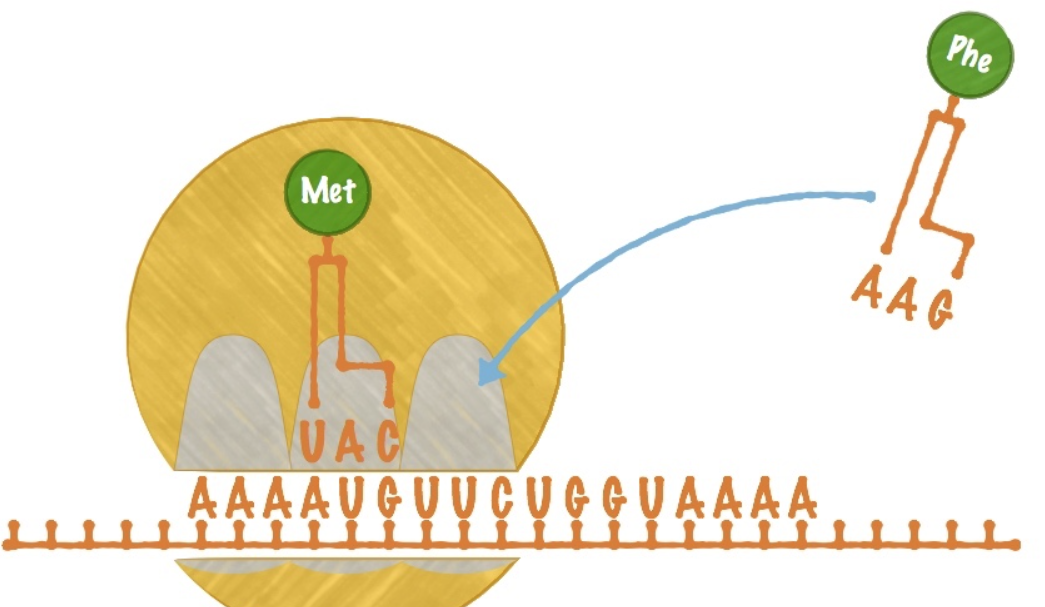
\includegraphics[width=0.5\linewidth]{Screenshot 2023-10-05 23.14.36.png}
    
    
\end{figure}


\end{questions}
\end{document}
